\chapter{Numerical methods}

\label{chp:numerical_methods}

\graphicspath{{images/numerical_methods/}}

\todo{introduction}

\section{Lare1D}

Lare3d, an abbreviation of LAgragian-REmap 3d, is a numerical scheme used to solve partial differential equations like those found in fluid dynamics and magnetohydrodynamics. The core idea of the scheme is to solve the equations on a grid in Lagrangian form, which involves a deformation of the grid, and then to remap the variables back to the original, Eulerian grid. This two-step process, combined with additional shock-capturing techniques such as flux limiters and shock viscosity, is extremely effective at capturing the kind of shocks that are generated in highly compressible, dynamic coronal simulations. It compares extremely well to Roe solvers when solving identical problems~\cite{arberStaggeredGridLagrangian2001}.

As a consequence of the Lagrangian step, the equations are solved in a much simpler form than if they were to be solved in equivalent Eulerian form. The disadvantage of this is that a complex remap step must be introduced. However, once the remap problem is solved, and it is only a complicated but tractable problem of geometry, it is not necessary to change the step when the physics are changed. Like other finite-volume methods, the method requires only local communication, that is a computation on a single cell requires only information from nearby cells. This locality reduces the overhead associated with communication between nodes when implementing the method on large clusters and makes the method viable for large-scale simulations. 

Here, we present the implementation and tests of a 1D LARE scheme applied to the inviscid, compressible Euler equations. We then provide an summary of the MHD code Lare3D~\cite{arberStaggeredGridLagrangian2001} which is used to perform the numerical experiments detailed in the rest of the thesis. 

\subsection{The physical model}
For an ideal, inviscid fluid we use the 1D Euler equations, describing the change in density $\rho$ due to expansion or compression of the fluid through spatial change in the flow velocity $u$,
\begin{equation}
  \frac{D \rho}{Dt} + \rho\frac{\partial u}{\partial x} = 0,\\
  \label{eqn-lare1d-density}
\end{equation}
the change in velocity due to a difference in pressure $p$,
\begin{equation}
  \frac{D u}{Dt} + \frac{1}{\rho}\frac{\partial p}{\partial x} = 0,\\
  \label{eqn-lare1d-velocity}
\end{equation}
the change in internal energy $\varepsilon$ due to expansion or compression,
\begin{equation}
  \frac{D \varepsilon}{Dt} + \frac{p}{\rho}\frac{\partial u}{\partial x} = 0,\\
  \label{eqn-lare1d-energy}
\end{equation}
and an ideal equation of state,
\begin{equation}
  p = \varepsilon\rho(\gamma - 1).
  \label{eqn-lare1d-equation-of-state}
\end{equation}
Including an equation of state simplifies the problem and negates the need to solve the density equation directly. Use has been made of the Lagrangian derivative, defined as
\begin{equation}
  \frac{D }{Dt} \equiv \frac{\partial}{\partial t} + (\vec{u} \cdot \nabla).
\end{equation}
It describes how a quantity within a parcel of fluid changes as that parcel is advected by the flow. 

\subsection{Discretisation} 

\begin{figure}[t]
    \hfill
    \begin{subfigure}{0.3\textwidth}
      \centering
      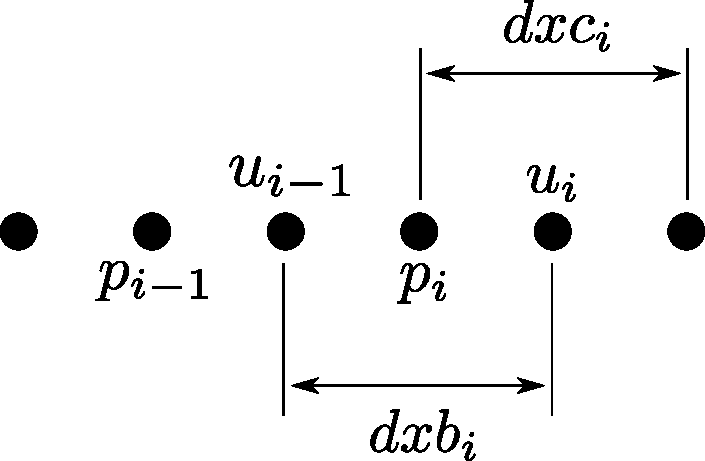
\includegraphics[width=1.0\linewidth]{staggered_grid.pdf}
      \caption{Staggered grid}%
      \label{fig:staggered_grid}
    \end{subfigure}
    \hfill
    \begin{subfigure}{0.49\textwidth}
      \includegraphics[width=\linewidth]{remap.png}
      \caption{Remap step}%
      \label{fig:remap}
    \end{subfigure}
    \caption{\ref{fig:staggered_grid} Staggered grid showing velocity located at cell-boundaries and pressure located at cell-centres, and~\ref{fig:remap} illustration of the deformation of the grid during the Lagrangian step and the remapping of variables back to the original grid during the remap step.}
\label{fig:grid_and_remap}%
\end{figure}

As illustrated in figure~\ref{fig:staggered_grid}, the grid on which the variables are defined is staggered, that is the velocity is defined at the boundary of the cells, and all other variables are defined at cell centres. This is in contrast to collocated grids where all variables are defined at the same locations on a single grid. Without staggering, our specific choice of the spatial discretisation of derivatives would result in two sets of decoupled equations, one associated with even indices and one with odd. This decoupling can cause a numerical instability often called the checkerboard problem and is a common numerical issue in computational fluid dynamics generally~\cite{ferzigerComputationalMethodsFluid2002}. Additionally, it has been found that the use of a staggered grid can improve the accuracy of a finite-difference scheme with little extra computational overhead~\cite{rojanaratanangkulePerformanceHighOrder2015}. However, a staggered grid is more complex to implement, requiring careful consideration of the precise locations of derivatives and the handling of two separate grids. 

Due to the staggered grid, we define the derivative of the velocity at the centre of a cell to be the first-order, central finite-difference of the velocity at the boundaries,
\begin{equation}
  {\left( \frac{\partial u}{\partial x} \right)}_i = \frac{u_i - u_{i-1}}{dxb_i},
  \label{}
\end{equation}
and similarly we define the derivative of pressure (or any of the other cell-centred variables) at the boundaries,
\begin{equation}
  {\left( \frac{\partial p}{\partial x} \right)}_i = \frac{p_i - p_{i-1}}{dxc_i}.
  \label{}
\end{equation}

\subsection{The Lagrangian step}
The Lagrangian step uses a kind of predictor-corrector scheme to advance the system one timestep. Each timestep is split into two substeps, the first calculating an approximation of the pressure, and the second using this pressure to advance all other variables to the next full timestep. Here we start at timestep $n$, the predictor step advances the pressure to timestep $n+1/2$ and then finally the corrector step advances the remaining variables to timestep $n+1$.

It's unclear whether this type of numerical integration scheme could be considered a ``true'' predictor-corrector scheme, or instead an explicit Runge-Kutta method. Predictor-corrector schemes typically provide a prediction of the system at a single advanced timestep using an explicit method and then correct the values at that timestep using an implicit method~\cite{butcherNumericalMethodsOrdinary2004}. In contrast, an explicit Runge-Kutta scheme advances the system using multiple approximate solutions at intermediate timesteps. It is my opinion that this scheme is better described as a Runge-Kutta method. However the full 3D MHD code, Lare3D, and its corresponding literature~\cite{arberStaggeredGridLagrangian2001} uses predictor-corrector nomenclature, so those terms are used here for consistency with~\cite{arberStaggeredGridLagrangian2001}.

\paragraph{The predictor step}
It can be shown by Taylor expansion that calculating $u^{n+1}$, $\varepsilon^{n+1}$ and $\rho^{n+1}$ to second order only requires calculating $p^{n+1/2}$ to first order. Using equation~\eqref{eqn-lare1d-equation-of-state},
\begin{equation}
  p_i^{n+1/2} = \varepsilon_i^{n+1/2}(\gamma-1)\rho_i^{n+1/2}.
  \label{eqn-predictor-pressure}
\end{equation}
The energy density at the half timestep is calculated from the discretisation of equation~\eqref{eqn-lare1d-energy},
\begin{equation}
  \varepsilon_i^{n+1/2} = \varepsilon_i^{n} - \frac{dt}{2} \frac{1}{\rho_i^n} \frac{u_i^n - u_{i-1}^n}{dxb_i^n}p_i^{n+1/2}.
  \label{eqn-predictor-energy}
\end{equation}
Since mass is conserved, the change in density is related to the change in volume in the following way,
\begin{equation}
  \rho_i^{n+1} = \frac{\rho_i^{n}}{\Delta},
\end{equation}
where $\Delta = dxb_i^{n+1}/dxb_i^{n}$ is the fractional change in volume between the current and future timestep. In this case, the density at the half timestep is found by calculating the updated grid boundary separation,
\begin{equation}
  dxb_i^{n+1/2} = dxb_i^n + \frac{dt}{2}(u_i^n - u_{i-1}^n),
  \label{eqn-predictor-boundary-distance}
\end{equation}
and feeding this into the calculation of the volume change, and thus the updated density,
\begin{equation}
  \rho_i^{n+1/2} = \rho_i^n \frac{dxb_i^n}{dxb_i^{n+1/2}}.
  \label{eqn-predictor-density}
\end{equation}

\paragraph{The corrector step}
\label{sec-corrector-step}
After the half-timestep pressure has been calculated, the velocity, energy and grid spacing are all advanced to time index $n+1$. The velocity is calculated through the discretisation of equation~\eqref{eqn-lare1d-velocity},
\begin{equation}
  u_i^{n+1} = u_i^n - dt \frac{1}{\rho^n_{i+1/2}}\frac{p^{n+1/2}_{i+1} - p^{n+1/2}_i}{dxc_i^n},
  \label{}
\end{equation}
where the density at the cell boundary $\rho_{i+1/2}$ is found via a mass-conserving interpolation,
\begin{equation}
  \rho_{i+1/2} = \frac{dxb_i \rho_i + dxb_{i+1}\rho_{i+1}}{dxb_i + dxb_{i_1}}.
  \label{eqn-lagrangian-density-interpolation}
\end{equation}
It should be noted that half timestep values for $\rho$ and $dxb$ have not been used here. This is a consequence of the product $\rho_i dxb_i$ being conserved throughout the Lagrangian step, that is $\rho_i^{n+1/2} dxb_i^{n+1/2} = \rho_i^n dxb_i^n$.

In order to advance the remaining variables we require the half timestep value for the velocity, calculated using a simple temporal average,
\begin{equation}
  u_i^{n+1/2} = \frac{1}{2}(u_i^{n} + u_i^{n+1}).
  \label{}
\end{equation}
This allows the advancement of the energy to the next full timestep, calculated from the discretisation of equation~\eqref{eqn-lare1d-energy},
\begin{equation}
  \varepsilon_i^{n+1} = \varepsilon_i^{n} - dt \frac{1}{\rho_i^n} \frac{u_i^{n+1/2} - u_{i-1}^{n+1/2}}{ dxb_i^n}p_i^{n+1/2}.
  \label{}
\end{equation}
We update the grid separation,
\begin{align}
  dxb_i^{n+1} &=  dxb_i^n + dt(u_i^{n+1/2} - u_{i-1}^{n+1/2}),\\
  dxc_i^{n+1} &=  (dxb_i^{n+1} + dxb_{i+1}^{n+1})/2,
  \label{eqn-lagrangian-grid-update}
\end{align}
and finally the density,
\begin{equation}
  \rho_i^{n+1} = \rho_i^n \frac{dxb_i^n}{dxb_i^{n+1}}.
  \label{}
\end{equation}

\subsection{The remap step}
Updating the variables during the Lagrangian step distorts the grid from its original state. The remap step rectifies this by mapping the variables from the distorted Lagrangian grid to the original, undeformed grid. We initially remap the density before switching to a mass coordinate to remap the energy and velocity. Using the mass coordinate has the benefit of conserving mass during the remap step.

The remapping process is a purely geometrical exercise and the problem-specific physics are contained entirely in the Lagrangian step. This is advantageous when applying the scheme to a general set of problems since once the remap step is realised and implemented, the entire scheme can be adapted to a specific problem by changing only the equations in the Lagrangian step. Major changes in geometry such as a different coordinate system or the inclusion of periodic boundary conditions would, however, require some adaptation in the remap step. Although the implementation detailed in this chapter takes one Lagrangian step per remap step, some LARE implementations take many Lagrangian steps, continuing until the distortion of the grid becomes greater than some criteria, only then performing a remap step. The following remap process could be used to remap a distortion created over multiple Lagrangian steps and only requires data from before and after the entire deformation of the grid. 

\paragraph{The Density Remap}
Due to the flow, after a single Lagrangian step an amount of mass $dM_i$ leaves the $i$-th Eulerian cell via the right hand side and an amount $dM_{i-1}$ enters via the left hand side, as shown in figure~\ref{fig:mass_movement}. The mass remaining in the cell is given by
\begin{equation}
  \rho^{n+1}_i dxb_i = \rho'_i dxb'_i - dM_i + dM_{i-1},
  \label{eqn-remap-mass-in-cell}
\end{equation}
where we use $\rho_i$ without the dash to denote the density before the Lagrangian step, the dashed variable $\rho'_i$ to denote the density of the $i$-th cell after a Lagrangian step and $\rho_i^{n+1}$ to denote the final density after the remap step. Note that the grid spacing is remapped to its original Eulerian value so $dxb^{n+1}_i = dxb_i$. By conservation of mass during the Lagrangian step, $\rho_i dxb_i = \rho'_i dxb'_i$ and equation \eqref{eqn-remap-mass-in-cell} becomes
\begin{equation}
  \rho^{n+1}_i = \rho_i + \frac{1}{dxb_i} (dM_{i-1} - dM_i).
  \label{eqn-remap-density}
\end{equation}

\begin{figure}[t]
  \centering
  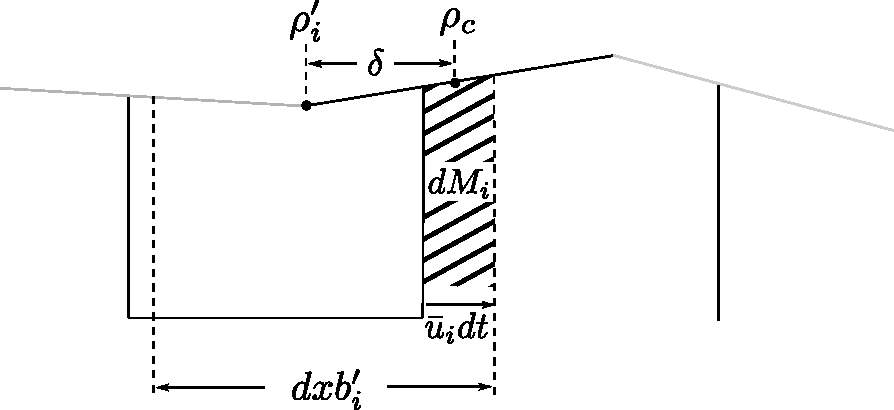
\includegraphics[width=0.7\linewidth]{mass_movement.pdf}
  \caption{Advection of mass from one cell to an adjacent cell.}%
  \label{fig:mass_movement}
\end{figure}

As can be seen from figure~\ref{fig:mass_movement}, since we are considering $\rho_i$ to be piecewise linear, the mass leaving the right hand side is given by
\begin{equation}
  dM_i = \rho_c \bar{u}_i dt,
\end{equation}
where $\bar{u}$ denotes the velocity of the boundary which, as seen in equation \eqref{eqn-lagrangian-grid-update}, is given by the half-timestep velocity $u_i^{n+1/2}$. If multiple Lagrangian timesteps were being taken, the single distance $\bar{u}_i dt$ would be replaced by the total distance that the boundary moved. The density of the part of the cell that has moved beyond the right hand side boundary is given by
\begin{equation}
  \rho_c = \rho_i' + \delta \frac{\partial \rho_i'}{\partial x'}.
\end{equation}
Geometrically we can see that,
\begin{align}
  \delta =  \frac{1}{2} dxb_i' - \frac{1}{2} \bar{u}_i dt = \frac{1}{2} dxb_i'(1-\psi),
\end{align}
where we have extracted  written $\psi = \bar{u}_i dt / dxb_i'$. The calculation of $\partial\rho_i'/ \partial x'$ is performed using a third-order upwind method, given by
\begin{equation}
  \label{eq:upwind_method}
D_i = 
\begin{cases}
\frac{2-\psi_i}{3} \frac{f_{i+1} - f_i}{dxb_i} + \frac{1+\phi_i}{3}\frac{f_i - f_{i-1}}{dxb_{i-1}}, \quad \bar{u_i} > 0,\\
\frac{2-\psi_i}{3} \frac{f_{i+1} - f_i}{dxb_i} + \frac{1+\phi_i}{3}\frac{f_{i+2} - f_{i+1}}{dxb_{i+1}}, \quad \bar{u_i} \leq 0.
\end{cases}
\end{equation}
The corresponding method for variables located at the boundaries uses the same formulae but with $dxb$ replaced by $dxc$. As is explained in section~\ref{sec:shock_capturing}, the naive application of this method can lead to numerical issues so, in practice, the gradient $D_i$ is limited using the flux limiter described in section~\ref{sec-flux-limiters}. Thus we can calculate the mass leaving the right hand side, 
\begin{equation}
dM_i = \left( \rho_i' + \frac{1}{2}dxb'_i(1-\psi) \frac{\partial \rho_i'}{\partial x'} \right) \bar{u}_i dt,
\label{eqn-remap-mass-diff}
\end{equation} 
and using equation \eqref{eqn-remap-density} we complete the remap of the density.

\subsection{The Specific Energy Density Remap}
Since we have already calculated the mass leaving the $i$-th Eulerian cell, $dM_i$, we can work purely in mass coordinates instead of $x$-coordinates, which has the advantage of naturally conserving mass in the remap of the specific energy density. The distance $dxb$ in mass coordinates $\xi$ is given by
\begin{equation}
  d\xi_i = \rho_i dxb_i = \rho_i' dxb_i'.
\end{equation}

Now we can follow a nearly identical thought process to the density remap, beginning with noting that the energy left in the $i$-th Eulerian cell after a Lagrangian step is taken is given by
\begin{equation}
  \varepsilon_i^{n+1} dxb_i \rho_i^{n+1} = \varepsilon_i' dxb_i' \rho_i' + dE_{i-1} - dE_i,
\end{equation}
where $dE_i$ is the amount of energy being advected out of the cell through the right hand side boundary and $dE_{i-1}$ is the energy advected in through the left hand side boundary. Rearranging for $\varepsilon_i^{n+1}$, 
\begin{equation}
  \varepsilon_i^{n+1}  = \frac{1}{dxb_i \rho_i^{n+1}}(\varepsilon_i' dxb_i \rho_i + dE_{i-1} - dE_i),
  \label{eqn-remap-specific-energy-density}
\end{equation}
where we have again made use of mass conservation, $dxb_i \rho_i = dxb_i' \rho_i'$.

Drawing a similar figure to~\ref{fig:mass_movement} leads us to geometrically calculate $dE_i$ to be
\begin{equation}
  dE_i = \varepsilon_c dM_i.
\end{equation}
It can be seen that
\begin{equation}
  \varepsilon_c = \varepsilon_i' + \delta \frac{\partial \varepsilon_i'}{\partial xi},
\end{equation}
and
\begin{equation}
  \delta = \frac{1}{2}d\xi_i - \frac{1}{2}dM_i.
\end{equation}
Hence, 
\begin{equation}
  dE_i = \left( \varepsilon_i' + \frac{1}{2}\frac{\partial \varepsilon_i'}{\partial \xi} (d\xi_i - dM_i) \right)dM_i.
\end{equation}
Since we are storing $\varepsilon$ in $x$-space, not in mass space, we use the fact that
\begin{equation}
  d\xi_i \frac{\partial \varepsilon_i'}{\partial \xi} = dxb_i\rho_i \frac{\partial \varepsilon_i'}{\partial \xi} = dxb_i \frac{\partial \varepsilon_i}{\partial x}
\end{equation}
to rewrite $dE_i$ as
\begin{equation}
  dE_i = \left( \varepsilon_i' + \frac{1}{2}dxb_i\frac{\partial \varepsilon_i'}{\partial x} \left( 1 - \frac{dM_i}{\rho_i dxb_i} \right) \right)dM_i,
  \label{eqn-remap-energy-difference}
\end{equation}
where calculation of $\partial \varepsilon_i'/\partial\xi$ is again done using flux limiters and is discussed in section~\ref{sec-flux-limiters}. This final equation coupled with equation \eqref{eqn-remap-specific-energy-density} completes the specific energy density remap.

\subsection{The velocity remap}
\label{sec-remap-velocity}
The velocity remap is nearly identical to the specific energy density remap completed within equations \eqref{eqn-remap-specific-energy-density} and \eqref{eqn-remap-energy-difference} so a derivation will not be given, however since the velocity is defined at cell centres, some of the relevant variables must be interpolated. The two equations required to remap the velocity are 
\begin{align}
  dU_i &= \left( u_i' + \frac{1}{2}dxc_i\frac{\partial u_i'}{\partial x} \left( 1 - \frac{dM_{i+1/2}}{\rho_{i+1/2} dxc_i} \right) \right)dM_{i+1/2},\\
  u_i^{n+1}  &= \frac{1}{dxc_i \rho_{i+1/2}^{n+1}}(u_i' dxc_i \rho_{i+1/2} + dU_{i-1} - dU_i),
\end{align}
where we have replaced the boundary distance $dxb$ with the cell centre distance $dxc$, mass is interpolated using a simple average, $dM_{i+1/2} = (dM_{i} + dM_{i+1})/2$ and the density is interpolated using equation \eqref{eqn-lagrangian-density-interpolation}. Once again, the derivative $\partial u_i' / \partial x$ is found using flux limiters. 

\subsection{Constraints on the timestep}
Lagrangian-remap schemes are often considered to be unconditionally stable and do not have a CFL condition like many explicit numerical schemes~\cite{batesMultiplyUpstreamSemiLagrangianAdvective1982}. Despite this, the remap step detailed previously makes some assumptions about how the grid deforms during the Lagrangian step, namely a gridpoint cannot be advected more than one grid separation away from its original position. This condition appears similar to a CFL condition and restricts the timestep $dt$ to
\begin{equation}
  \label{eq:grid_condition1}
  dt < \frac{dxb_i}{|u_i|}\quad \forall i.
\end{equation}
Without this condition a large enough velocity could deform the grid so much that the remap step is not able to correctly remap the variables. With a more complex remap step, the assumptions about the grid deformation and corresponding timestep constraints could be relaxed.

\subsection{Expansion to 3D}
The 3D version of this remap step is of course much more involved geometrically but it follows an analogous path. Cell boundaries would be represented as cell planes and the boundary valued variables defined either on cell face centres or cell corners. In~\cite{arberStaggeredGridLagrangian2001} the cell face centres are chosen due to the cell corners introducing unnecessarily complex geometrical problems.

\todo{this needs extending}

\section{Shock capturing techniques}
\label{sec:shock_capturing}

In hyperbolic systems of PDEs such as that given in equations~\ref{eqn-lare1d-density}--\ref{eqn-lare1d-energy} discontinuous solutions like shock waves are valid. While shock waves (or shocks) do have some physical width in real systems, they are typically so thin compared to the larger scales of the system that they are treated as discontinuities mathematically. Numerical solvers which aim to represent a solution on a finite grid of points struggle to provide enough resolution to accurately resolve a shock. When under-resolved, high-resolution numerical solvers may overestimate the shock, creating an overshoot in the solution and introducing spurious oscillations in the wake of the shock, known as the carbuncle phenomenon~\cite{rodionovArtificialViscosityCure2019}. Two methods of dealing with these unwanted oscillations are used in this code: flux limiters, which restricts spatial gradients and maintains monotonicity, and shock viscosity, which acts to better resolve the shock by spreading it over numerous grid points. The use of these techniques in both the 1D code and lare3d are detailed here.

\subsection{Flux Limiters}
\label{sec-flux-limiters}

Flux limiters are numerical tools applied to high-resolution schemes to reduce the spurious oscillations associated with such schemes by restricting the flux through some numerical interface. In practice, this often involves the restriction of spatial gradients, so flux limiters are often called slope limiters. A wide variety of flux limiters have been developed, however attention here is restricted to total variation diminishing (TVD) schemes, specifically that of van Leer~\cite{vanleerUltimateConservativeDifference1997}. For a review of other TVD schemes, see~\cite{zhangReviewTVDSchemes2015}, and for a review of the related essentially non-oscillatory scheme, see~\cite{shuHighOrderENO1999a}. 

To measure the degree of oscillation in a quantity $q$, the total variation of the discretised quantity is defined as
\begin{equation}
  \label{eq:total_variation}
TV(q) = \sum_{i=1}^{N} | q_i - q_{i-1} |.
\end{equation}
Any oscillation which is generated in the wake of a shock generates local maxima and minima which increase the total variation. TVD schemes aim to maintain, or at least decrease, this measure. As a result, a shock, which by its nature is monotonic, should remain monotonic when a TVD scheme is applied. A good TVD scheme should also only weakly affect maxima and minima which are true features of the solution.

\begin{figure}[t]
  \centering
  \includegraphics[width=0.4\linewidth]{van_leer_flux_limiter}
  \caption{The gradient at index $i$, $D_i$ (solid line) is limited to the gradient $D_i^{mono}$ (heavy solid line) to ensure the value of $f_i$ extrapolated to the left-hand boundary of the cell is less than the average value of the neighbouring cell, $f_{i-1}$. This diagram is a modified reproduction of that found in~\cite{vanleerUltimateConservativeDifference1997}.}%
  \label{fig:van_leer_flux_limiter}
\end{figure}

Consider the cells shown in figure~\ref{fig:van_leer_flux_limiter}, where we wish to calculate the gradient of the quantity $f$ at the index $i$. This scheme is valid regardless of method of discretisation of the gradient so we label this gradient $D_i$ for now. The monotonicity requirement of van Leer requires the value of $f$, extrapolated to the boundary to the right to be less than the average value of that cell, $f_{i+1}$. For a cell centred variable, this condition can be written
\begin{equation}
  \label{eq:flux_limiter1}
f_i + \tfrac{1}{2}D_i^{mono} dxb_i < f_{i+1} \quad \text{or} \quad D_i^{mono} < 2 (f_{i+1} - f_i) / dxb_i.
\end{equation}
Correspondingly, the value of $f$ extrapolated to the left must be greater than $f_{i-1}$ giving
\begin{equation}
  \label{eq:flux_limiter2}
f_i - \tfrac{1}{2}D_i^{mono} dxb_i > f_{i-1} \quad \text{or} \quad D_i^{mono} < 2 (f_{i} - f_{i-1}) / dxb_i.
\end{equation}
When the gradients are reversed, a similar set of conditions exists to maintain monotonicity.

These conditions on $D_i^{mono}$ are met if
\begin{equation}
  \label{eq:flux_limiter3}
D_i^{mono} = s \min(|D_i|, 2 | f_{i+1} - f_i |, 2 |f_i - f_{i-1}|),
\end{equation}
where
\begin{equation}
  \label{eq:flux_limiter4}
s =
\left\{
	\begin{array}{ll}
		\text{sign}(D_i)  & \mbox{if } \text{sign}(D_i) = \text{sign}(f_{i+1} - f_i) = \text{sign}(f_{i} - f{i-1}) \\
		0 & \mbox{otherwise}
	\end{array}
\right.
\end{equation}
The action of this second part of the limiter, represented by $s$, can be understood by considering a few example cases. The outputted gradient is only non-zero when the gradient $D_i$ aligns with neighbouring gradients, that is the signs of the gradients are all equal, as is the case in figure~\ref{fig:van_leer_flux_limiter}. In this case, the outputted slope is either the original slope if the monotonicity conditions are met, or a first-order approximation otherwise, as given by equation~\ref{eq:flux_limiter3}. In all other cases, for example where the cell $i$ represents a maxima or minima, the outputted gradient is zero to ensure monotonicity.

\subsection{Shock Viscosity}

Shock viscosity (or artificial viscosity) is a method of artificially spreading the shock over multiple grid points, thus capturing the shock. An alternative to this, used particularly in supersonic aerodynamics, is the use of shock fitting techniques, where the location of the shock is determined numerically (or analytically if the location is known \emph{a priori}) and the grid shaped to fit the shock and align the discontinuity with the grid points~\cite{paciorriShockfittingTechnique2D2009}.

Mirroring the choice of shock viscosity used in lare3d~\cite{arberStaggeredGridLagrangian2001}, which is that of Wilkins~\cite{wilkinsUseArtificialViscosity1980a}, the artificial viscosity $q$ is taken to be
\begin{equation}
  \label{eq:artificial_viscosity}
q = c_1 \rho c_s | \Delta u | + c_2 \rho (\Delta u)^2,
\end{equation}
where $c_s^2 = \gamma p / \rho$ is the sound speed, $\Delta u$ is the difference in velocity across the shock, and $c_1$ and $c_2$ are constants to be optimised by experiment. This is an extension of the widely-used von Neumann-Richtmyer shock viscosity~\cite{vonneumannMethodNumericalCalculation1950}. The scalar $q$ is added to the thermal pressure during the predictor stage of the Lagrangian step. Since the artificial viscosity is modifying the pressure, the energy equation must gain an additional term incorporating the heat generated by the shock viscosity, which takes the form $-q\Delta u/\rho$. To ensure this term only heats, it should only be included where $\Delta u < 0$. 

In the full 3D code, the shock viscosity given in equation~\ref{eq:artificial_viscosity} is extended to include 3D, MHD shocks. The viscosity, now modelled as a tensor similar to that of Newtonian viscosity, takes the form
\begin{equation}
  \label{eq:3d_shock_viscosity}
\ten{\sigma}_{shock} = (c_1 \rho c_f L |s| + c_2 L^2 \rho s^2) \ten{W},
\end{equation}
where the scalar quantity $q$ has been modified to include $L$ and $s$ as the grid length and strain rate, both measured in the direction of the acceleration, and $c_f$ is the fast mode speed. For 1D hydrodynamic shocks, equation~\ref{eq:3d_shock_viscosity} reduces to equation~\ref{eq:artificial_viscosity}. Viscosity in this form has the advantage of being negligible everywhere except the locations where a compressional shock is present. Since shock viscosity applied in this way is a numerical tool originally developed for hydrodynamic purposes, it is unclear if this an appropriate tool for use in MHD shocks, where the viscosity is intrinsically anisotropic. A more complex model of shock viscosity which includes the effect of the magnetic field while still adequately capturing shocks would be more appropriate. For this reason, the shock viscosity is turned off in all 3D numerical experiments in proceeding chapters, to ensure it does not influence the investigation of anisotropic viscosity. The shock viscosity is enabled in the 1D code described here, however.

\section{Implementation}
\subsection{Full recipe}
\paragraph{Predictor Step}
The corrector step requires only the pressure at the half-timestep $n+1/2$, thus for each grid point we temporarily calculate the energy, density and boundary distance at the half-timestep using equations \eqref{eqn-predictor-energy}, \eqref{eqn-predictor-density} and \eqref{eqn-predictor-boundary-distance} respectively, and feed these into the equation for pressure, \eqref{eqn-predictor-pressure} storing the result for use in the corrector step.

\paragraph{Corrector Step}
Looping over all grid points the updated velocity, velocity at half-timestep, density, energy and grid separations are all calculated and stored using the corrector equations given in \ref{sec-corrector-step}. These variables are all used in the remap step.

\paragraph{Remap Step}
Completing one cycle of the simulation, the density and energy are remapped back to the original Eulerian grid using equations \eqref{eqn-remap-density}, \eqref{eqn-remap-mass-diff}, \eqref{eqn-remap-energy-difference} and \eqref{eqn-remap-specific-energy-density}. Once the relevant interpolations are complete, the velocity remap is achieved using the equations given in section \ref{sec-remap-velocity}. It is during this stage that the flux limiters are used to obtain the derivatives of density, energy and velocity with respect to $x$.

\subsection{Language and library choice}
This example of a LARE scheme was implemented in C++, a language which effectively balances computational speed and usability. The \emph{getopt} and \emph{json} libraries were used to take input from a JSON file allowing for better runtime flexibility. The unit testing library \emph{Catch} was used as the testing framework. Since this is a one-dimensional problem with limited complexity, there was no need to include parallelism in the code, although due to the computations being well-localised, it would be reasonably simple to parallelise the code using similar approaches to those commonly applied to finite-difference and finite-volume codes. Some helper tools were also written in Python and running scripts in bash. Due to the mature numerical and plotting libraries available for Python, it is a natural choice of language for developing tools.

\section{Numerical test}

The code was tested using the Sod shock tube problem. The problem was used to run parameter studies over the two shock viscosity parameters to identify optimal values, values which minimise an error function. The optimal values found indicate that the linear shock viscosity term, the first term in equation~\ref{eq:artificial_viscosity}, is mostly sufficient for this problem. Other parameter choices give benefits that are unquantified by the chosen error function.

\begin{figure}[t]
  \centering
  \includegraphics[width=\linewidth]{sod_analytical_solution.pdf}
  \caption{Analytical solution to the Sod shock tube problem. The solution is separated into five regions: the left (L) and right (R) regions, which keep the values of the initial conditions; the right (1) and left (2) states on either side of the contact discontinuity, region 1 bounded to the right by the shock and region 2 to the left by the rarefaction wave; and the rarefaction wave itself (E).}%
  \label{fig:sod_analytical_solution}
\end{figure}

The code was tested using the Sod problem, a problem commonly used in testing compressible hydrodynamic codes which has a known analytical solution~\cite{sodSurveySeveralFinite1978}, shown in figure~\ref{fig:sod_analytical_solution}. The initial conditions for the problem is a discontinuity in both pressure and density at the location $x_0=0.5$,
\begin{equation}
  \label{eq:sod_problem_ic}
\begin{pmatrix}\rho _{L}\\p_{L}\\u_{L}\end{pmatrix}
=
\begin{pmatrix}1.0\\1.0\\0.0\end{pmatrix},
\begin{pmatrix}\rho _{R}\\p_{R}\\u_{R}\end{pmatrix}
=
\begin{pmatrix}0.125\\0.1\\0.0\end{pmatrix}.
\end{equation}

This large initial pressure jump generates three waves: a shock wave, a contact discontinuity and a rarefaction wave. Shock waves are the discontinuous limit of compressive waves, created as a result of flow velocities exceeding the local speed of sound. These can form spontaneously or as the result of a smooth compressive wave steepening. The states before and after the shock are connected by the Rankine-Hugoniot conditions, described in the proceeding paragraphs. Contact discontinuities are similar to shock waves, and are similarly governed by the Rankine-Hugoniot conditions, but only involve a jump in density, maintaining pressure equilibrium across the jump. Rarefaction (or expansion) waves are travelling regions of expanding medium, in contrast to a compressive wave. Such waves are often found in the wake of shocks, as is the case here. The rarefaction wave here travels leftwards. These three waves can be identified in figure~\ref{fig:sod_analytical_solution}.

\subsection{Analytical solution}

The analytical solution to the problem is found by splitting the solution into five parts, as described and shown in figure~\ref{fig:sod_analytical_solution}. The solution in regions R and L are the values set in the initial conditions. These known states can be connected to the unknown states in regions 1, 2 and E via the Rankine-Hugoniot conditions and the locations of the interfaces between the regions, $x_{1, 2, 3, 4}$ found by the method of characteristics. The Rankine-Hugoniot conditions for the Euler equations represent the conservation of mass, momentum and total energy across a discontinuity. These are written
\begin{equation}
  \label{eq:rk}
\begin{aligned}
  u_R - u_L &= s\left(\frac{1}{\rho_L} - \frac{1}{\rho_R}\right),\\
  p_R - p_L &= s(u_R - u_L),\\
  p_R u_R - p_L u_L &= s (E_R - E_L),\\
\end{aligned}
\end{equation}
where $s$ is the speed of the discontinuity, $E = \varepsilon + u^2/2$ is the total energy and the value of a variable to the right (left) of a discontinuity is given the subscript $R$ ($L$). For brevity I shall only state the analytical solution, however a full derivation can be found in~\cite{danailaIntroductionScientificComputing2006}.

The Mach number of the shock, $M_s = s/a_r$ is calculated via the implicit equation,
\begin{equation}
  \label{eq:mach_shock}
M_s - \frac{1}{M_s} = a_L \frac{\gamma + 1}{\gamma - 1} \left\{
1 - \left[
\frac{p_R}{p_L} \left(
\frac{2\gamma}{\gamma +1}M_s^2 - \frac{\gamma - 1}{\gamma +1} 
\right)
\right]^{\frac{\gamma - 1}{2\gamma}}
\right\},
\end{equation}
where $a_L = \sqrt{ \gamma p_L / \rho_L}$ is the local sound speed (defined similarly for other regions). For this problem, $M_s \approx 1.75$. This is used to calculate the pressure, density and velocity in region 1, found via the equations,
\begin{equation}
  \label{eq:sod_region1}
\begin{aligned}
\frac{p_1}{p_R} &= \frac{2\gamma}{\gamma + 1} M_s^2 - \frac{\gamma -1}{\gamma +1}\\
\frac{\rho_R}{\rho_1} &= \frac{2}{\gamma + 1} \frac{1}{M_s^2} + \frac{\gamma -1}{\gamma + 1},\\
u_1 &= \frac{2a_R}{\gamma + 1} \left( M_s - \frac{1}{M_s} \right).
\end{aligned}
\end{equation}
The velocity and pressure are equal across regions 1 and 2 and the density given by,
\begin{equation}
  \label{eq:sod_region2}
\rho = \rho_L \left( \frac{p_1}{p_L} \right)^{1/\gamma}.
\end{equation}
Within the rarefaction wave, the solution is given by,
\begin{equation}
  \label{eq:sod_regionE}
  \begin{aligned}
  p_E &= p_L \left( \frac{a}{a_L} \right)^{\frac{2\gamma}{\gamma-1}},\\
  \rho_E &= \frac{a^2}{\gamma p},\\
  u_E &= \frac{2}{\gamma +1} \left(a_L + \frac{x - x_0}{t}\right),
  \end{aligned}
\end{equation}
where $a = a_L - (\gamma-1)U/2$. The interfaces as defined in figure~\ref{fig:sod_analytical_solution} are given by
\begin{equation}
  \label{eq:sod_interfaces}
\begin{aligned}
x_1 &= x_0 - u_L t,\\
x_2 &= x_0 + (u_2 - a_2)t, \\
x_3 &= x_0 + u_2 t, \\
x_4 &= x_0 + M_s t.
\end{aligned}
\end{equation}

\subsection{Results}

To compare the error between resolutions, the total error $E_N$ is calculated as the $L_2$ norm of the difference between the full numerical and analytical solutions, normalised by the resolution,
\begin{equation}
  \label{eq:total_error}
E_N = \frac{1}{3N} \left(
\sum_{i=0}^{N-1} \norm{p_i - p(x_i)}_2
+ \sum_{i=0}^{N-1} \norm{\rho_i - \rho(x_i)}_2
+ \sum_{i=0}^{N-1} \norm{u_i - u(x_i)}_2 \right).
\end{equation}
This is only one possible way to evaluate a numerical solution. As shall be seen later, certain choices of parameters lead to numerical solutions which are closest to the analytical solution, that is they minimise $E_N$ for a given $N$, however other parameter choices better resolve features like steep gradients at the expense of an increase in global error. Since this is only a toy problem, I will not attempt to quantify such trade-offs here, opting to use the simple error measure given by equation~\ref{eq:total_error}.

\begin{figure}[t]
    \hfill
    \begin{subfigure}{0.49\textwidth}
      \centering
      \includegraphics[width=1.0\linewidth]{wide_shock_parameter_search.pdf}
      \caption{Wide parameter search}%
      \label{fig:wide_shock_parameter_search}
    \end{subfigure}
    \hfill
    \begin{subfigure}{0.49\textwidth}
      \includegraphics[width=\linewidth]{shock_parameter_search.pdf}
      \caption{Focused parameter search}%
      \label{fig:shock_parameter_search}
    \end{subfigure}
    \caption{Wide and focused parameter searches over the shock viscosity parameters $c_1$ and $c_2$, giving overall optimal values of $c_1 = 0.77$ and $c_2 = 0$ (crosses). The optimal values are calculated as those values which minimise the error given by equation~\ref{eq:total_error}. The colour is added to aid visibility and represents the error $E$. }
\label{fig:shock_parameter_searches}%
\end{figure}

\todo{change the labels in param fig to c1 and c2}

Figure~\ref{fig:shock_parameter_searches} shows surface plots of the error $E$ as a function of $c_1$ and $c_2$. Using a resolution of $N=500$, an initial parameter study of $2500$ points covering $c_1, c_2 \in [0, 10]$ was run and found optimal values of $c_1 = 0.8$ and $c_2 = 0$. A more focused study of $5000$ points further optimised these values to $c_1 = 0.77$ and $c_2 = 0$.

\begin{figure}[t]
  \centering
  \includegraphics[width=\linewidth]{shock_viscosity_variables.pdf}
  \caption{Solutions to the Sod problem for various values of the shock parameters at $t=0.2$ and for a resolution of $N=500$. The solution is plotted in the region $0.8 \leq x \leq 0.9$ to focus the shock itself. The analytical solution is also shown. Without shock viscosity the solution overshoots the true value behind the shock and does not effectively track the shock's position. Using the optimal values of $c_1 = 0.77$ and $c_2 = 0$ removes the overshoot and appears to track the approximate location of the shock well, but at the expense of the shock being smeared over many grid points. Using values of $c_1 = 0.1$ and $c_2 = 1.0$, as is done in~\cite{arberStaggeredGridLagrangian2001}, removes the overshoot, tracks the shock location better than no shock viscosity. Although using these values results in a more accurate, steeper shock gradient, the optimal values track the shock location more accurately.}%
  \label{fig:shock_viscosity_variables}
\end{figure}

While the optimal values minimise the error given in equation~\ref{eq:total_error}, using a lower $c_1$ and higher $c_2$ more accurately maintains the steep shock gradient, at the expense of less effectively tracking the shock location (figure~\ref{fig:shock_viscosity_variables}). As with many optimisation problems, choosing shock viscosity parameters requires balancing which aspects of the shock are considered crucial to a specific problem. 

\subsubsection{Effect of resolution}

\begin{figure}[t]
  \centering
  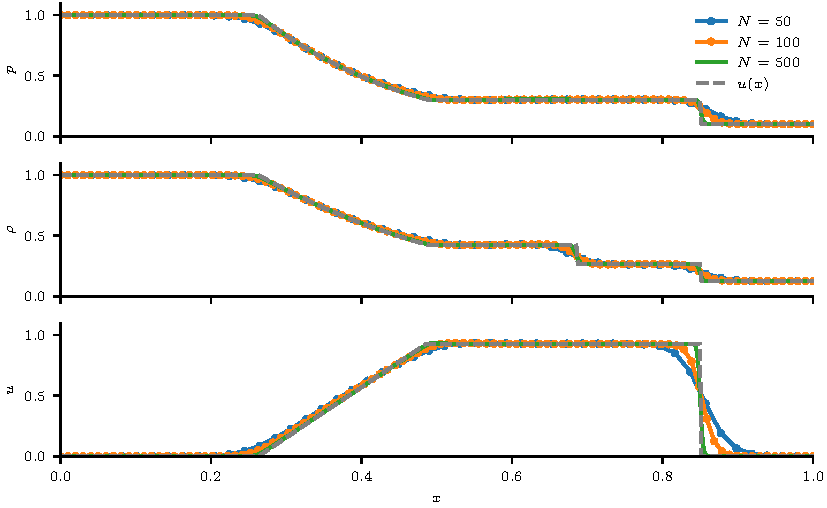
\includegraphics[width=1.0\linewidth]{resolution_study.pdf}
  \caption{Solutions to the Sod problem for resolutions of $N=50,\ 100,$ and $500$ (solid lines). The analytical solution is also shown (dotted line). The solutions at resolutions $N=50$ and $N=100$ are shown with dots at the grid point locations. The solution given for $t=0.2$ and the shock viscosity parameters are $c_1 = 0.77$ and $c_2 = 0$.}
  \label{fig:resolution_study}
\end{figure}

\begin{figure}[t]
  \centering
  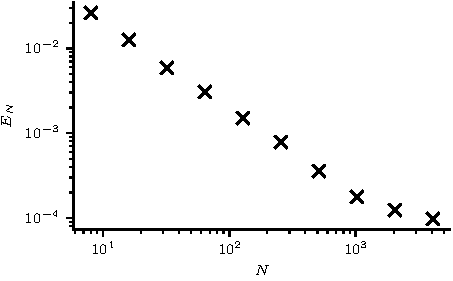
\includegraphics[width=0.5\linewidth]{effect_of_res_on_error.pdf}
  \caption{The effect of resolution on the solution accuracy. Each data point represents a simulation run with the optimal shock parameter values to $t=0.2$ using a resolution $N$. The error is calculated via equation~\ref{eq:total_error}.}%
  \label{fig:effect_of_res_on_error}
\end{figure}

The resolution affects the ability of the numerical scheme to adequately resolve discontinuities in the numerical solution. Figure~\ref{fig:resolution_study} shows three sample simulations at resolutions of $N=50$, $100$ and $500$. Although $N=500$ is a low resolution for 1D simulations, $500$ grid points per dimension in 3D MHD is a typical resolution. This simulation gives an indication of how well a fully 3D scheme might cope with shocks. Even with a low resolution of $N=50$, no features of the solution have been lost, although the discontinuities are artificially spread over a large distance.

Figure~\ref{fig:effect_of_res_on_error} shows the error $E_N$ as a function of resolution. The slope of the dependence suggests the global error is linearly dependent on the inverse of the resolution, instead of a quadratic dependence as expected from a second order scheme. This may be a result of the numerical scheme reverting to first order in the vicinity of discontinuities, or it may indicate an error in the code or the scheme. 

\section{Conclusion}

\todo{conclusion}
